
\section*{Problem  Set 4}

\subsection*{1.7 Group Actions}


\begin{mdframed}
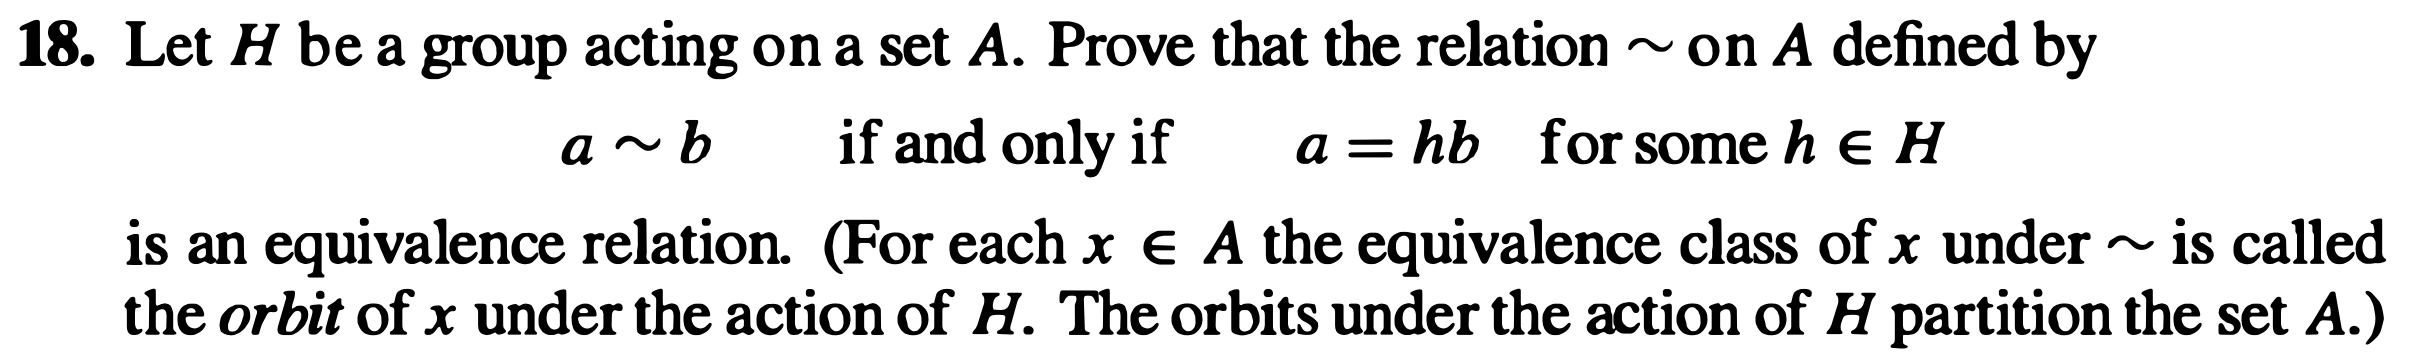
\includegraphics[width=400pt]{img/abstract-algebra--nf--4-bc71.png}
\end{mdframed}

\begin{intuition}
  Think of the elements of $A$ as vertices of a graph. There's an edge from $a_1$ to $a_2$ if some
  element of $h$ sends $a_1 \mapsto a_2$. Every multi-edge path has a corresponding single edge that goes
  to the same destination. To see that, imagine some path that involves multiple edges; but then
  there's also a single edge connecting the start and end point, given by the composition of the
  multiple edges (group closure means the composition is some other element in the group).

  It's reflexive because every group has an identity and this

  It's symmetric because $h^{-1}$ is the same edge as $h$ but with the opposite direction. It's
  transitive because as we said above, there's always a single edge that gets you to the same
  destination as any two-edge path.
\end{intuition}

\begin{proof}
  First note that $h$ acts on $A$ as a permutation, and $h^{-1}$ acts on $A$ as the the inverse of
  that permutation. Also note that the identity element acts as the identity permutation because
  the mapping from group elements to the permutations that they act as is a homomorphism, and a
  homomorphism always sends identity to identity.

  {\bf reflexive}\\
  $a \sim a$ since $a = 1a$.

  {\bf symmetric}\\
  If $a \sim b$ then $a = hb$ for some $h \in H$. Therefore $b = h^{-1}a$ hence $b \sim a$.

  {\bf transitive}\\
  If $a \sim b$ and $b \sim c$ then $a = h_1b$ and $b = h_2c$ for some $h_1, h_2 \in H$.
  Therefore $a = (h_1h_2)c$ hence $a \sim c$.
\end{proof}


\begin{mdframed}
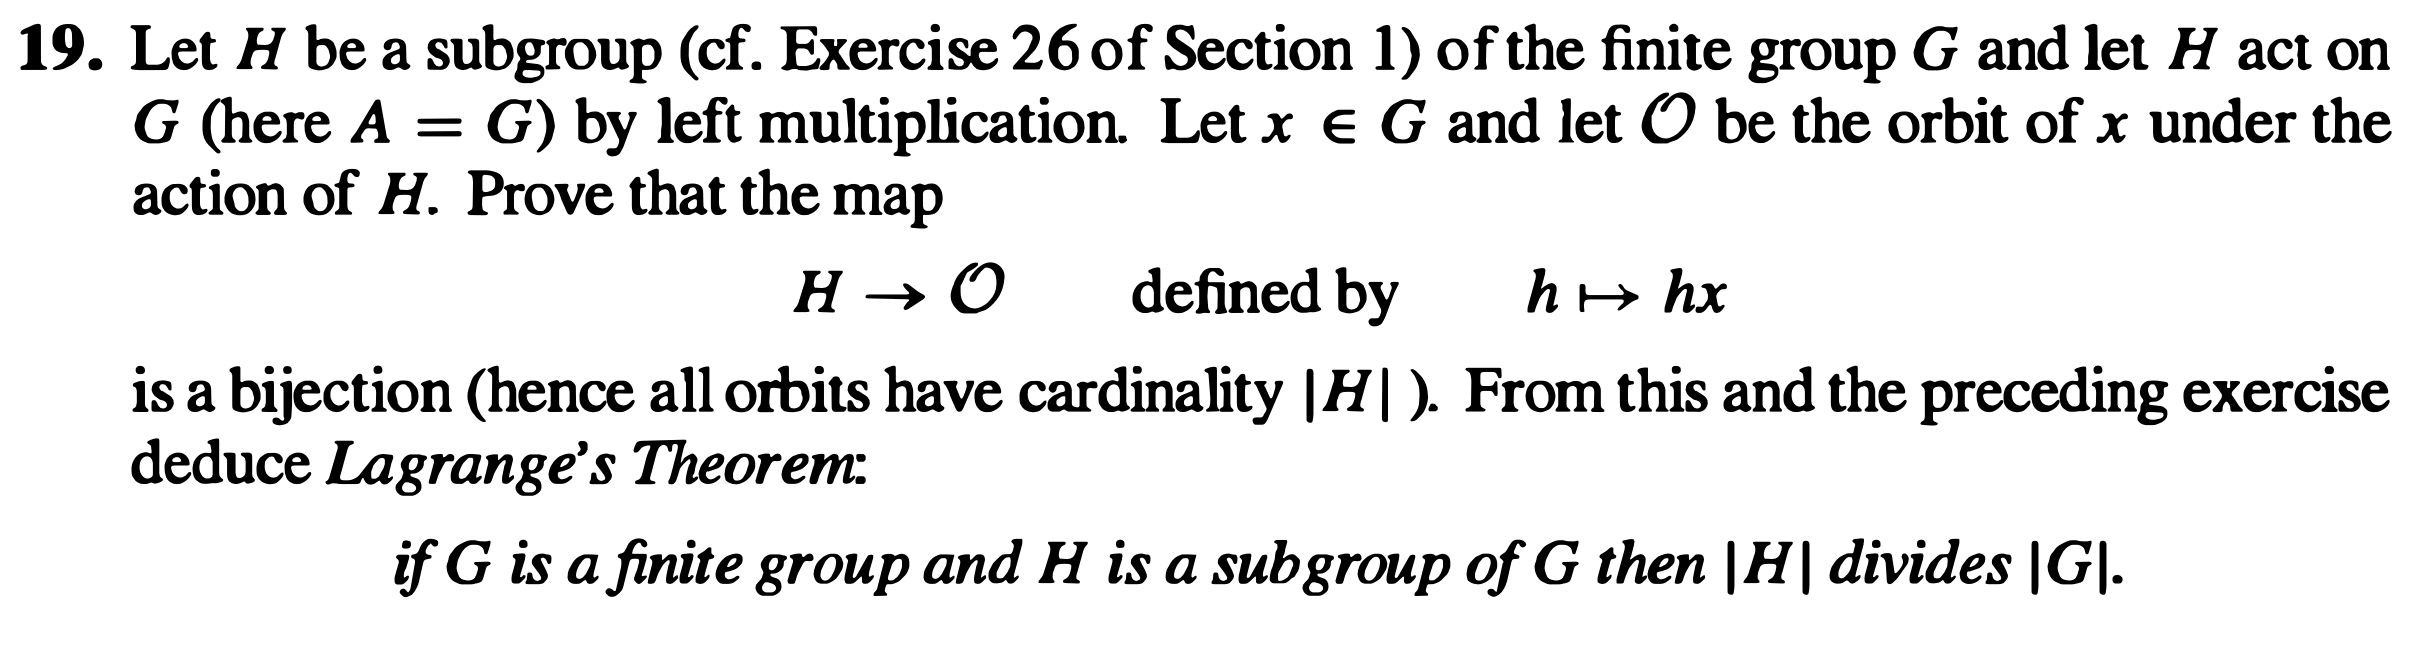
\includegraphics[width=400pt]{img/abstract-algebra--nf--4-4140.png}
\end{mdframed}

\begin{intuition}
  The map $\varphi$ in question sends $h$ to some element $hx$ of the orbit of $x$ under $H$.
  To get back, right-multiply by $x^{-1}$.

\end{intuition}

\begin{proof}
  Let $\varphi: H \to \mathcal O$ be the map defined by $h \mapsto hx$.

  The map $\psi: \mathcal O \to H$ defined by $g \mapsto gx^{-1}$ is a left inverse for $\varphi$,
  since $(\psi\varphi)(h) = \psi(\varphi(h)) = (hx)x^{-1} = h$, showing that $\psi\varphi = 1_H$, and also a right inverse
  for $\varphi$, since $(\varphi\psi)(g) = \varphi(\psi(g)) = (gx^{-1})x = g$, showing that $\varphi\psi = 1_G$.

  Therefore $\varphi$ is a bijection, since it has an inverse.

  Therefore the orbit of $x$ under the action of $H$ has cardinality $|H|$ and, since $x$ was
  arbitrary, this is true for the orbit of any $x \in G$ under the action of $H$.

  Since the orbits are equivalence classes, they partition $G$. Therefore $|G| = k|H|$ where $k$ is
  the number of distinct orbits.

  This argument required no assumptions beyond the premise that $H$ is a subgroup of a finite
  group $G$, hence Lagrange's Theorem:

  {\it if $H$ is a subgroup of a finite group $G$, then $H$ divides $|G$}


  ~\\
.
\end{proof}

\begin{mdframed}
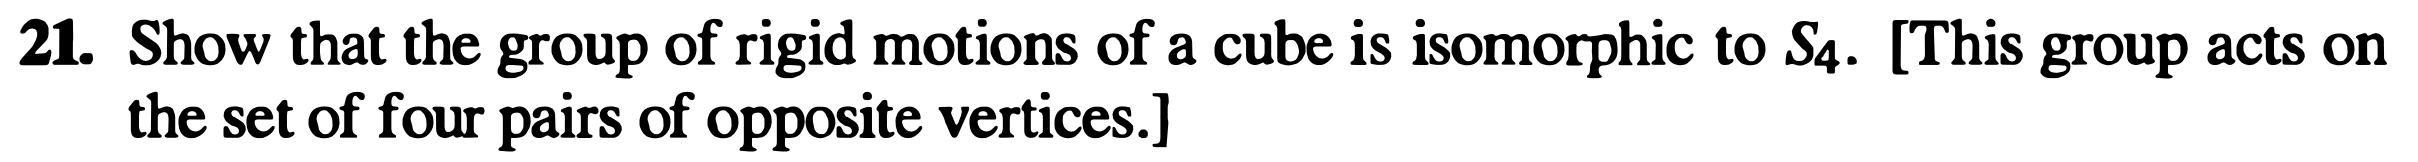
\includegraphics[width=400pt]{img/abstract-algebra--nf--4-0e63.png}
\end{mdframed}

{\it In case the terminology is unfamiliar, a "rigid motion" means a rotation or a reflection;
this group has the same relationship to the cube that the group $D_{2n}$ has to a regular n-gon.}

\begin{proof}
  Let $B$ be the set of $4$ pairs of opposite vertices of a cube, let $G$ be the group of rigid
  motions of a cube, acting on $B$, and let $\psi: G \to S_B$ be the permutation representation of the
  action of $G$ on $B$.

  We have $|S_B| = 4! = 24$ and also $|G| = 24$ (look at the cube face-on; after a rigid motion you
  are looking at one of the $6$ faces and that face is in one of its $4$ rotational
  configurations).

  Furthermore, every rigid motion other than the identity acts on $B$ as a non-identity
  permutation. To see this, consider the $4$ vertices of the face you are initially looking at.
  Unless the rigid motion is the identity then all $4$ of them have moved. [...needs more...]

  Therefore $\ker \psi = \{1\}$, hence $\psi$ is injective, and also an isomorphism since
  $|G| = |S_B|$, and since $S_B \cong S_4$ and isomorphism is a transitive relation, we have the
  desired result.
\end{proof}



\begin{mdframed}
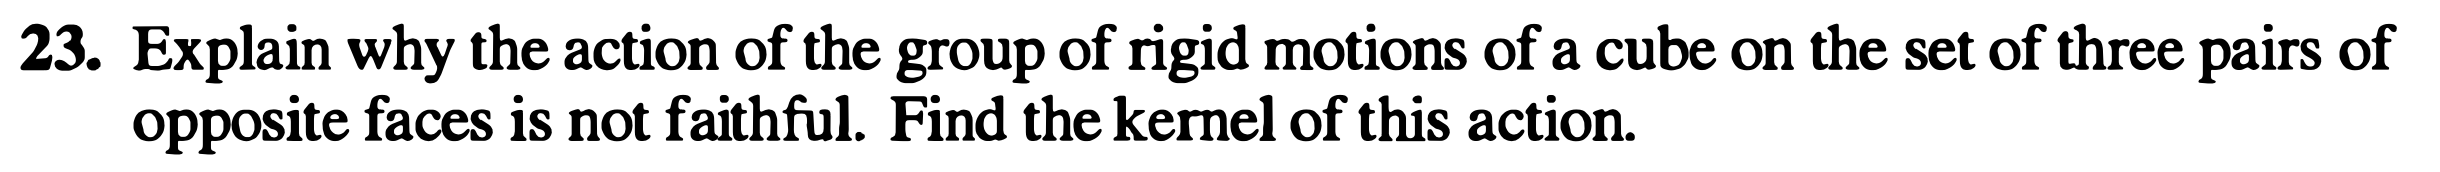
\includegraphics[width=400pt]{img/abstract-algebra--nf--4-5a92.png}
\end{mdframed}

\begin{proof}
  Let $B$ be a set of $3$ pairs of opposite vertices of a cube. Then $|S_B| = 3! = 6 < 24 = |G|$,
  hence any map $G \to S_B$ is non-injective, hence the permutation representation of $G$ acting
  on $B$ is non-injective, which is the definition of a non-faithful action.

  The kernel of this action is the set of pairs $(g, b)$ such that $gb = b$.

 union of $\{(I_G, b) ~|~ b \in B\}$ and $\{(r_b, )\}$
\end{proof}


\begin{mdframed}
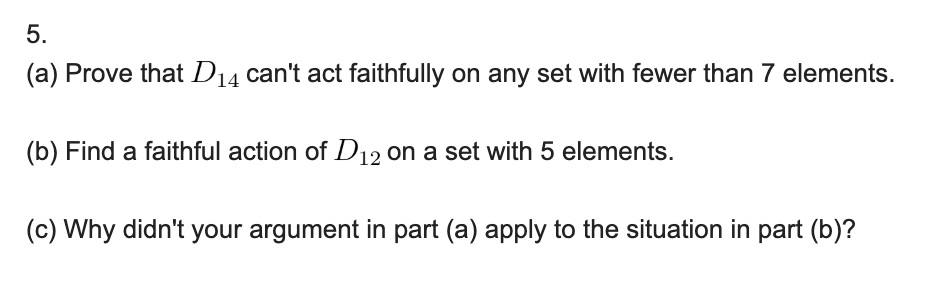
\includegraphics[width=400pt]{img/abstract-algebra--nf--4-1b73.png}
\end{mdframed}


\begin{mdframed}
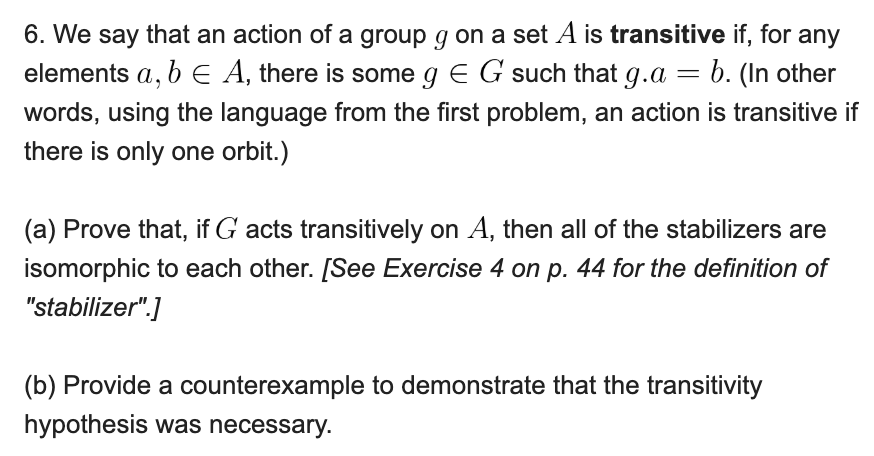
\includegraphics[width=400pt]{img/abstract-algebra--nf--4-50ae.png}
\end{mdframed}
